\section{IP}
\subsection{Capturing packets from an execution of traceroute}
    \subsubsection*{Problems}
    \begin{enumerate}[label=\bfseries Problem \arabic*:,leftmargin=*,labelindent=1em]
    %%%%%%%%%%%%%%%%%%%%%%%%%%%%%%%%%%%%%%%%%%%%%%%%% Problem 3-1
        \item Select the first ICMP Echo Request message sent by your computer, 
        and expand the Internet Protocol part of the packet in the packet details window.
        What is the IP address of your computer?\\[0.2mm]
        \soln IP address : 192.168.86.61
    %     \vspace{-4mm}  
        \begin{figure}[!h]\centering
        \hspace{15mm}  
    		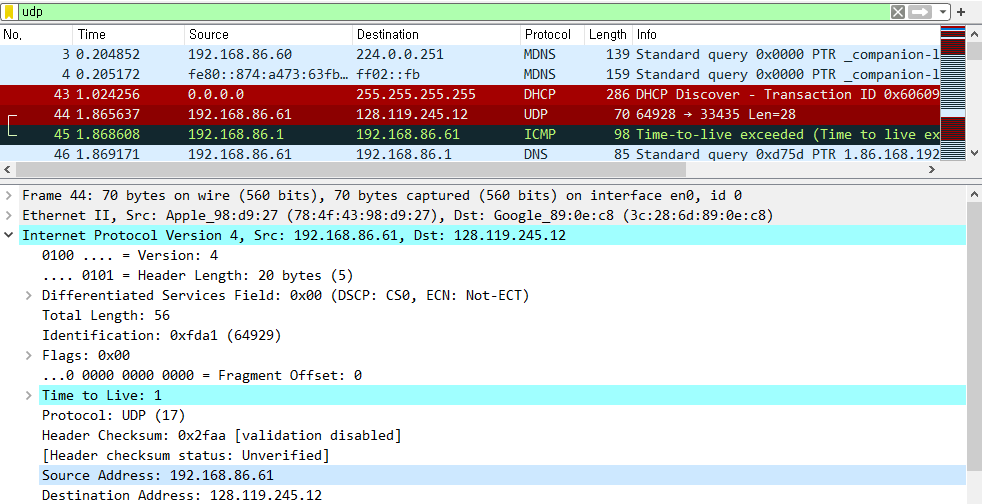
\includegraphics[width=.85\textwidth]{image/week02/3-1-1.png}
    		\caption{\footnotesize Problem 3-1's screenshot : }
    		\vspace{-10pt}
        \end{figure}
    %%%%%%%%%%%%%%%%%%%%%%%%%%%%%%%%%%%%%%%%%%%%%%%%% Problem 3-2
        \item Within the IP packet header, what is the value in the upper layer protocol field?\\[0.2mm]
        \soln
    %     \vspace{-4mm}  
        \begin{figure}[!h]\centering
        \hspace{15mm}  
    		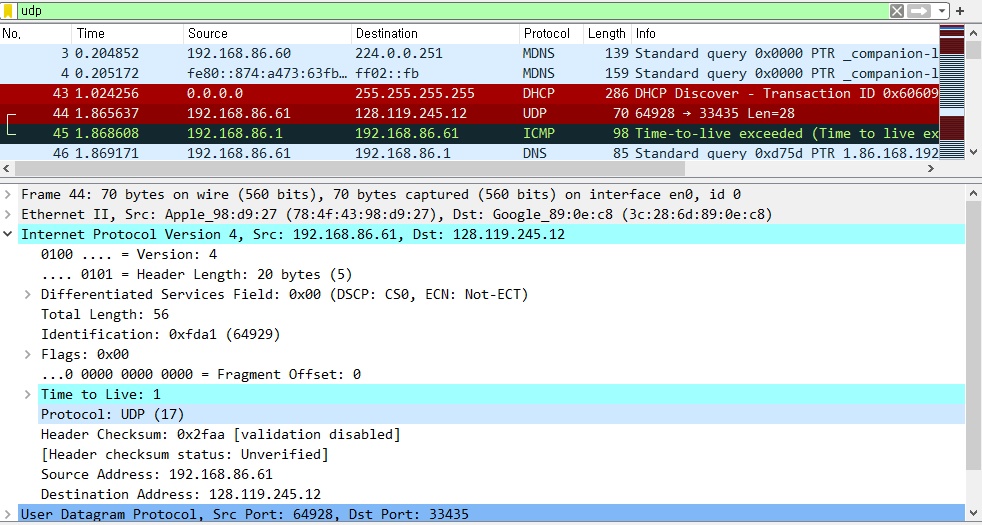
\includegraphics[width=.85\textwidth]{image/week02/3-2-1.png}
    		\caption{\footnotesize Problem 3-2's screenshot : }
    		\vspace{-10pt}
        \end{figure}
    %%%%%%%%%%%%%%%%%%%%%%%%%%%%%%%%%%%%%%%%%%%%%%%%% Problem 3-3
        \item How many bytes are in the IP header?\\[0.2mm]
        \soln
    %     \vspace{-4mm}  
        \begin{figure}[!h]\centering
        \hspace{15mm}  
    		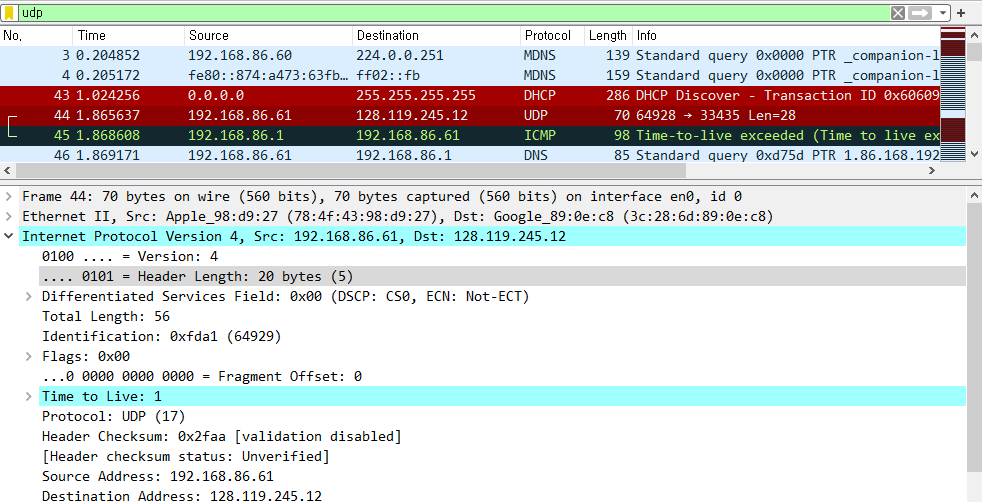
\includegraphics[width=.85\textwidth]{image/week02/3-3-1.png}
    		\caption{\footnotesize Problem 3-3's screenshot : }
    		\vspace{-10pt}
        \end{figure}
% \newpage
    %%%%%%%%%%%%%%%%%%%%%%%%%%%%%%%%%%%%%%%%%%%%%%%%% Problem 3-4
        \item How many bytes are in the payload of the IP datagram? Explain how you determined the number of payload bytes.\\[0.2mm]
        \soln
    %     \vspace{-4mm}  
        \begin{figure}[!h]\centering
        \hspace{15mm}  
    		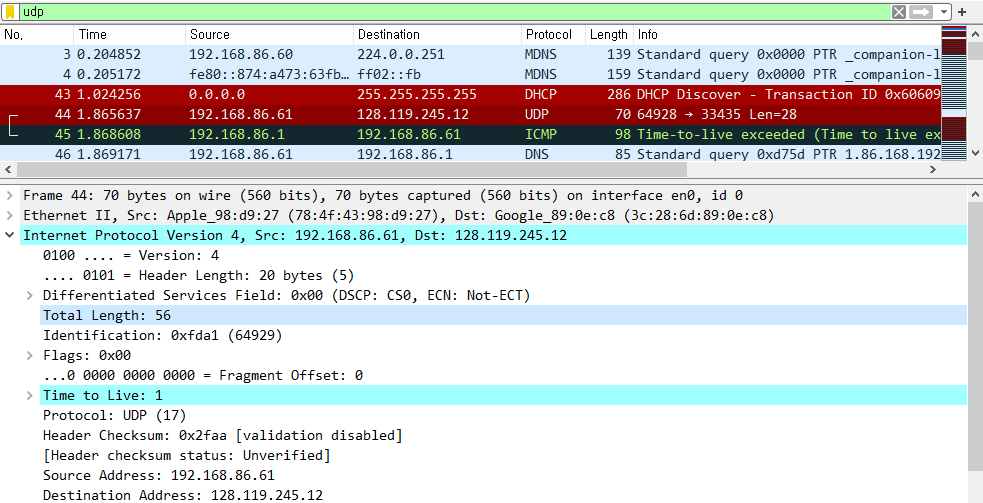
\includegraphics[width=.85\textwidth]{image/week02/3-4-1.png}
    		\caption{\footnotesize Problem 3-4's screenshot : }
    		\vspace{-10pt}
        \end{figure}
    %%%%%%%%%%%%%%%%%%%%%%%%%%%%%%%%%%%%%%%%%%%%%%%%% Problem 3-5
        \item Has this IP datagram been fragmented? 
        Explain how you determined whether or not the datagram has been fragmented.\\[0.2mm]
        \soln
    %     \vspace{-4mm}  
        \begin{figure}[!h]\centering
        \hspace{15mm}  
    		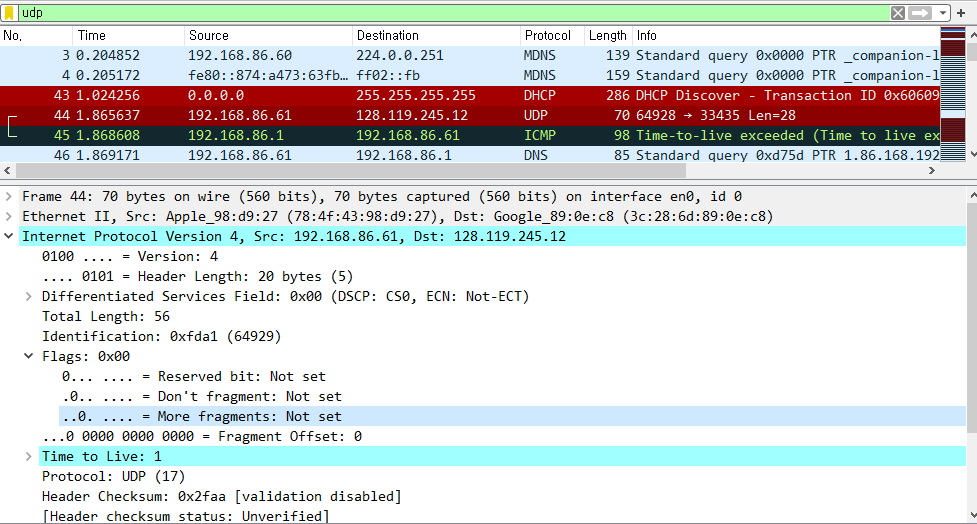
\includegraphics[width=.85\textwidth]{image/week02/3-5-1.png}
    		\caption{\footnotesize Problem 3-5's screenshot : }
    		\vspace{-10pt}
        \end{figure}
    \end{enumerate}
\newpage